\documentclass[11pt]{article}
\usepackage[utf8]{inputenc}
\usepackage[T1]{fontenc}
\usepackage{textcomp}
\usepackage[margin=1in]{geometry}
\usepackage{amsmath,amssymb,amsthm}
\usepackage{graphicx}
\usepackage{hyperref}
\usepackage{listings}
\usepackage{xcolor}
\usepackage{booktabs}
\usepackage{enumitem}

\definecolor{codebg}{RGB}{248,248,248}
\lstset{
  basicstyle=\ttfamily\small,
  backgroundcolor=\color{codebg},
  frame=single,
  breaklines=true,
  showstringspaces=false,
  keywordstyle=\color{blue!70!black},
  commentstyle=\color{green!50!black},
  stringstyle=\color{red!70!black},
  numbers=none,
  language=Python,
}

% Style for full-source listings in the appendix
\lstdefinestyle{appendixsrc}{
  basicstyle=\ttfamily\scriptsize,
  backgroundcolor=\color{codebg},
  frame=single,
  breaklines=true,
  showstringspaces=false,
  keywordstyle=\color{blue!70!black},
  commentstyle=\color{green!50!black},
  stringstyle=\color{red!70!black},
  numbers=left,
  numberstyle=\tiny\color{gray},
  numbersep=6pt,
  stepnumber=1,
  language=Python,
  columns=fullflexible,
  upquote=true,
  tabsize=4,
}

\title{ESE 650: Learning in Robotics --- Homework 4}
\author{Jinhao You \\ \texttt{you7@seas.upenn.edu}}
\date{Spring 2025}

\begin{document}
\maketitle

\section*{Time Spent}
\begin{itemize}[leftmargin=*]
    \item Problem 1 (MJPC): 30 minutes
    \item Problem 2 (PPO): 10 hours
\end{itemize}

%==============================================================================
\section{Problem 1 --- MuJoCo MPC Library (25 pts)}

\subsection*{(a) Installation}
Built MJPC from source following the README:
\begin{lstlisting}[language=bash]
git clone https://github.com/google-deepmind/mujoco_mpc.git
cd mujoco_mpc && mkdir build && cd build
cmake ..
make -j
\end{lstlisting}
Resulting binary: \texttt{build/bin/mjpc}.

\subsection*{(b) Cartpole, Acrobot, Walker}
Screenshots in Fig.~\ref{fig:mjpc-3systems} (also archived in
\texttt{hw4/p1/}). Each panel shows the simulator on the left and the
right-side telemetry pane (top: total cost decomposed by term;
middle: per-actuator action history; bottom: planner internals such
as gradient norm or sample diversity).

\paragraph{Cartpole.} The \texttt{cartpole} task uses the
\emph{Gradient} planner (visible in the Agent panel). The pole has
been driven essentially upright; the cart sits very close to the
target track and the recorded \texttt{Total Cost} on the right pane
is $\approx 0.002$, which is essentially the noise floor. The
\texttt{Actions} pane is also flat at zero --- once the pole is
balanced the gradient planner only injects tiny corrective torques.

\paragraph{Acrobot.} Acrobot uses the \emph{Sampling} planner with a
horizon of $2$ time units. The screenshot captures the moment the
lower link has built enough momentum to swing the upper link past
horizontal --- the system is on its way to the inverted equilibrium.
The cost trace on the right has dropped from an initial $\approx
100$ down to $\approx 1.5$, and the actions show the planner
delivering large coordinated torque pulses.

\paragraph{Walker (Humanoid Walk).} The walker model
(\texttt{humanoid\_walk}) uses Sampling-based MPC with separate
Pelvis, Feet, Posture, Velocity and Control cost terms (visible in
the Task pane on the left). The total cost has dropped to $\approx
1.3$ and individual cost terms (Velocity, Posture) are visibly
falling. The humanoid is mid-stride with one leg lifted, demonstrating
that the planner is actively cycling actions in a gait pattern rather
than holding a static pose.

\begin{figure}[h]
\centering
\begin{tabular}{cc}
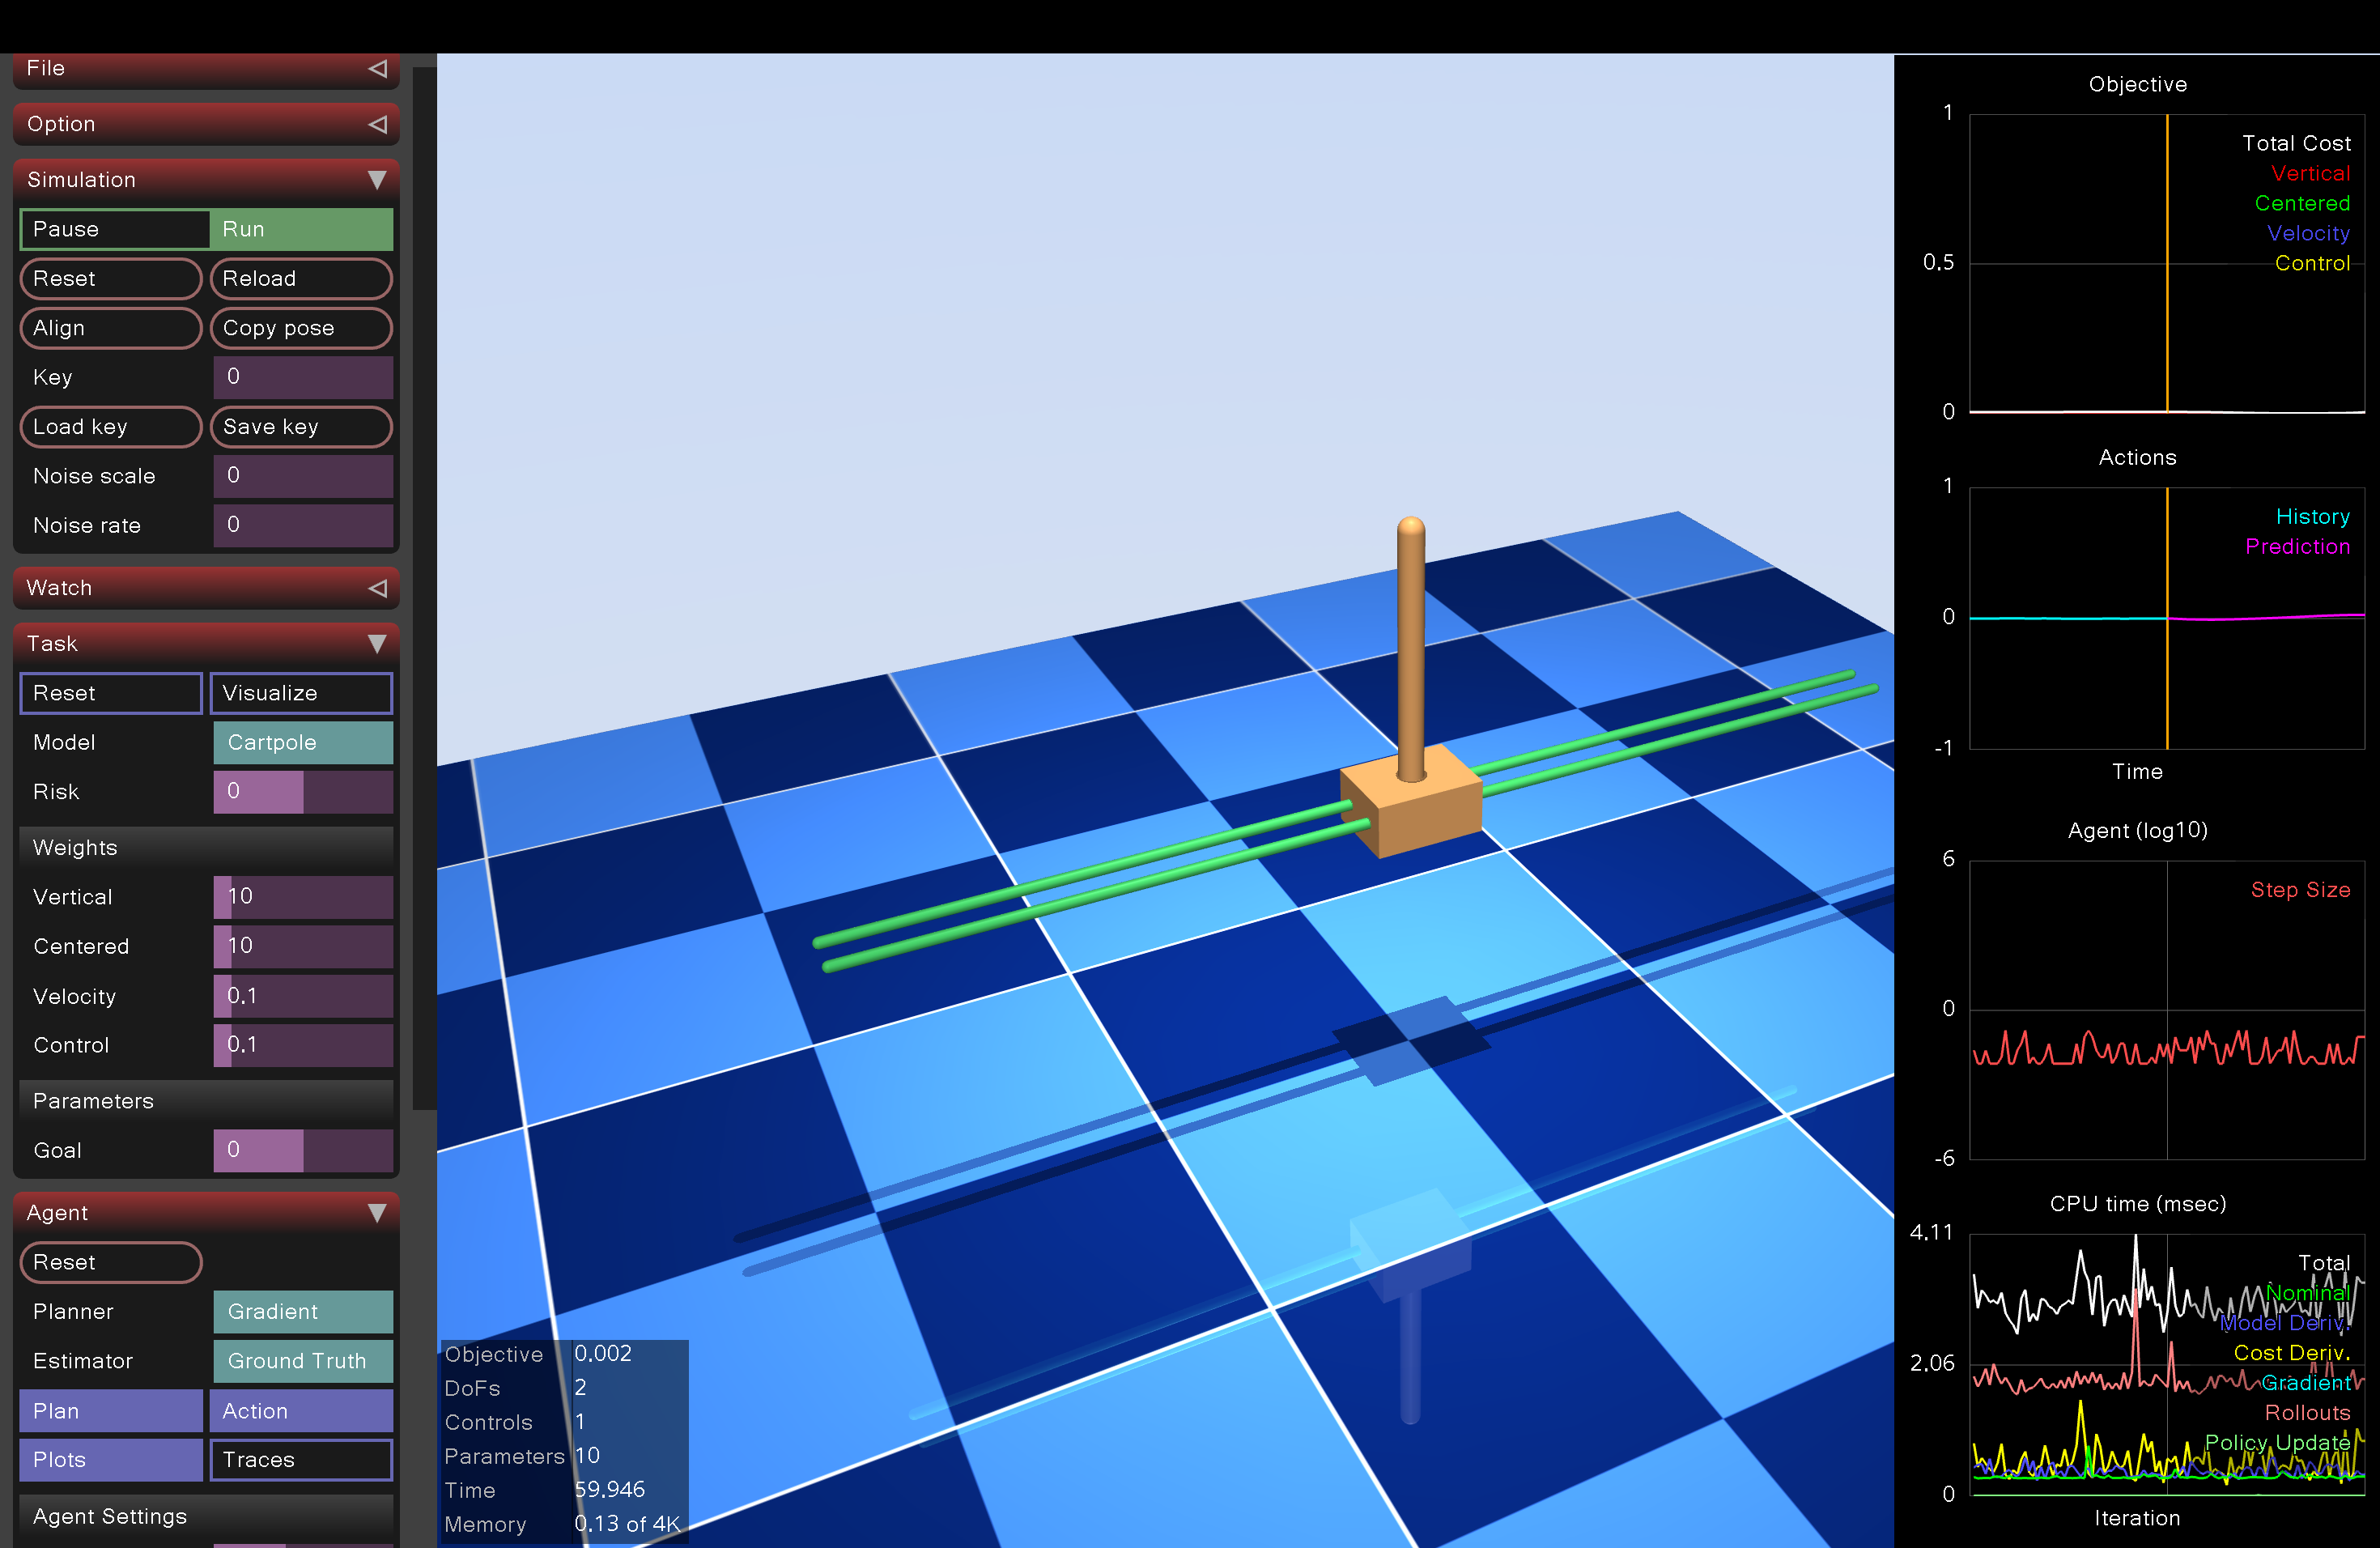
\includegraphics[width=0.46\textwidth]{p1/cartpole.png} &
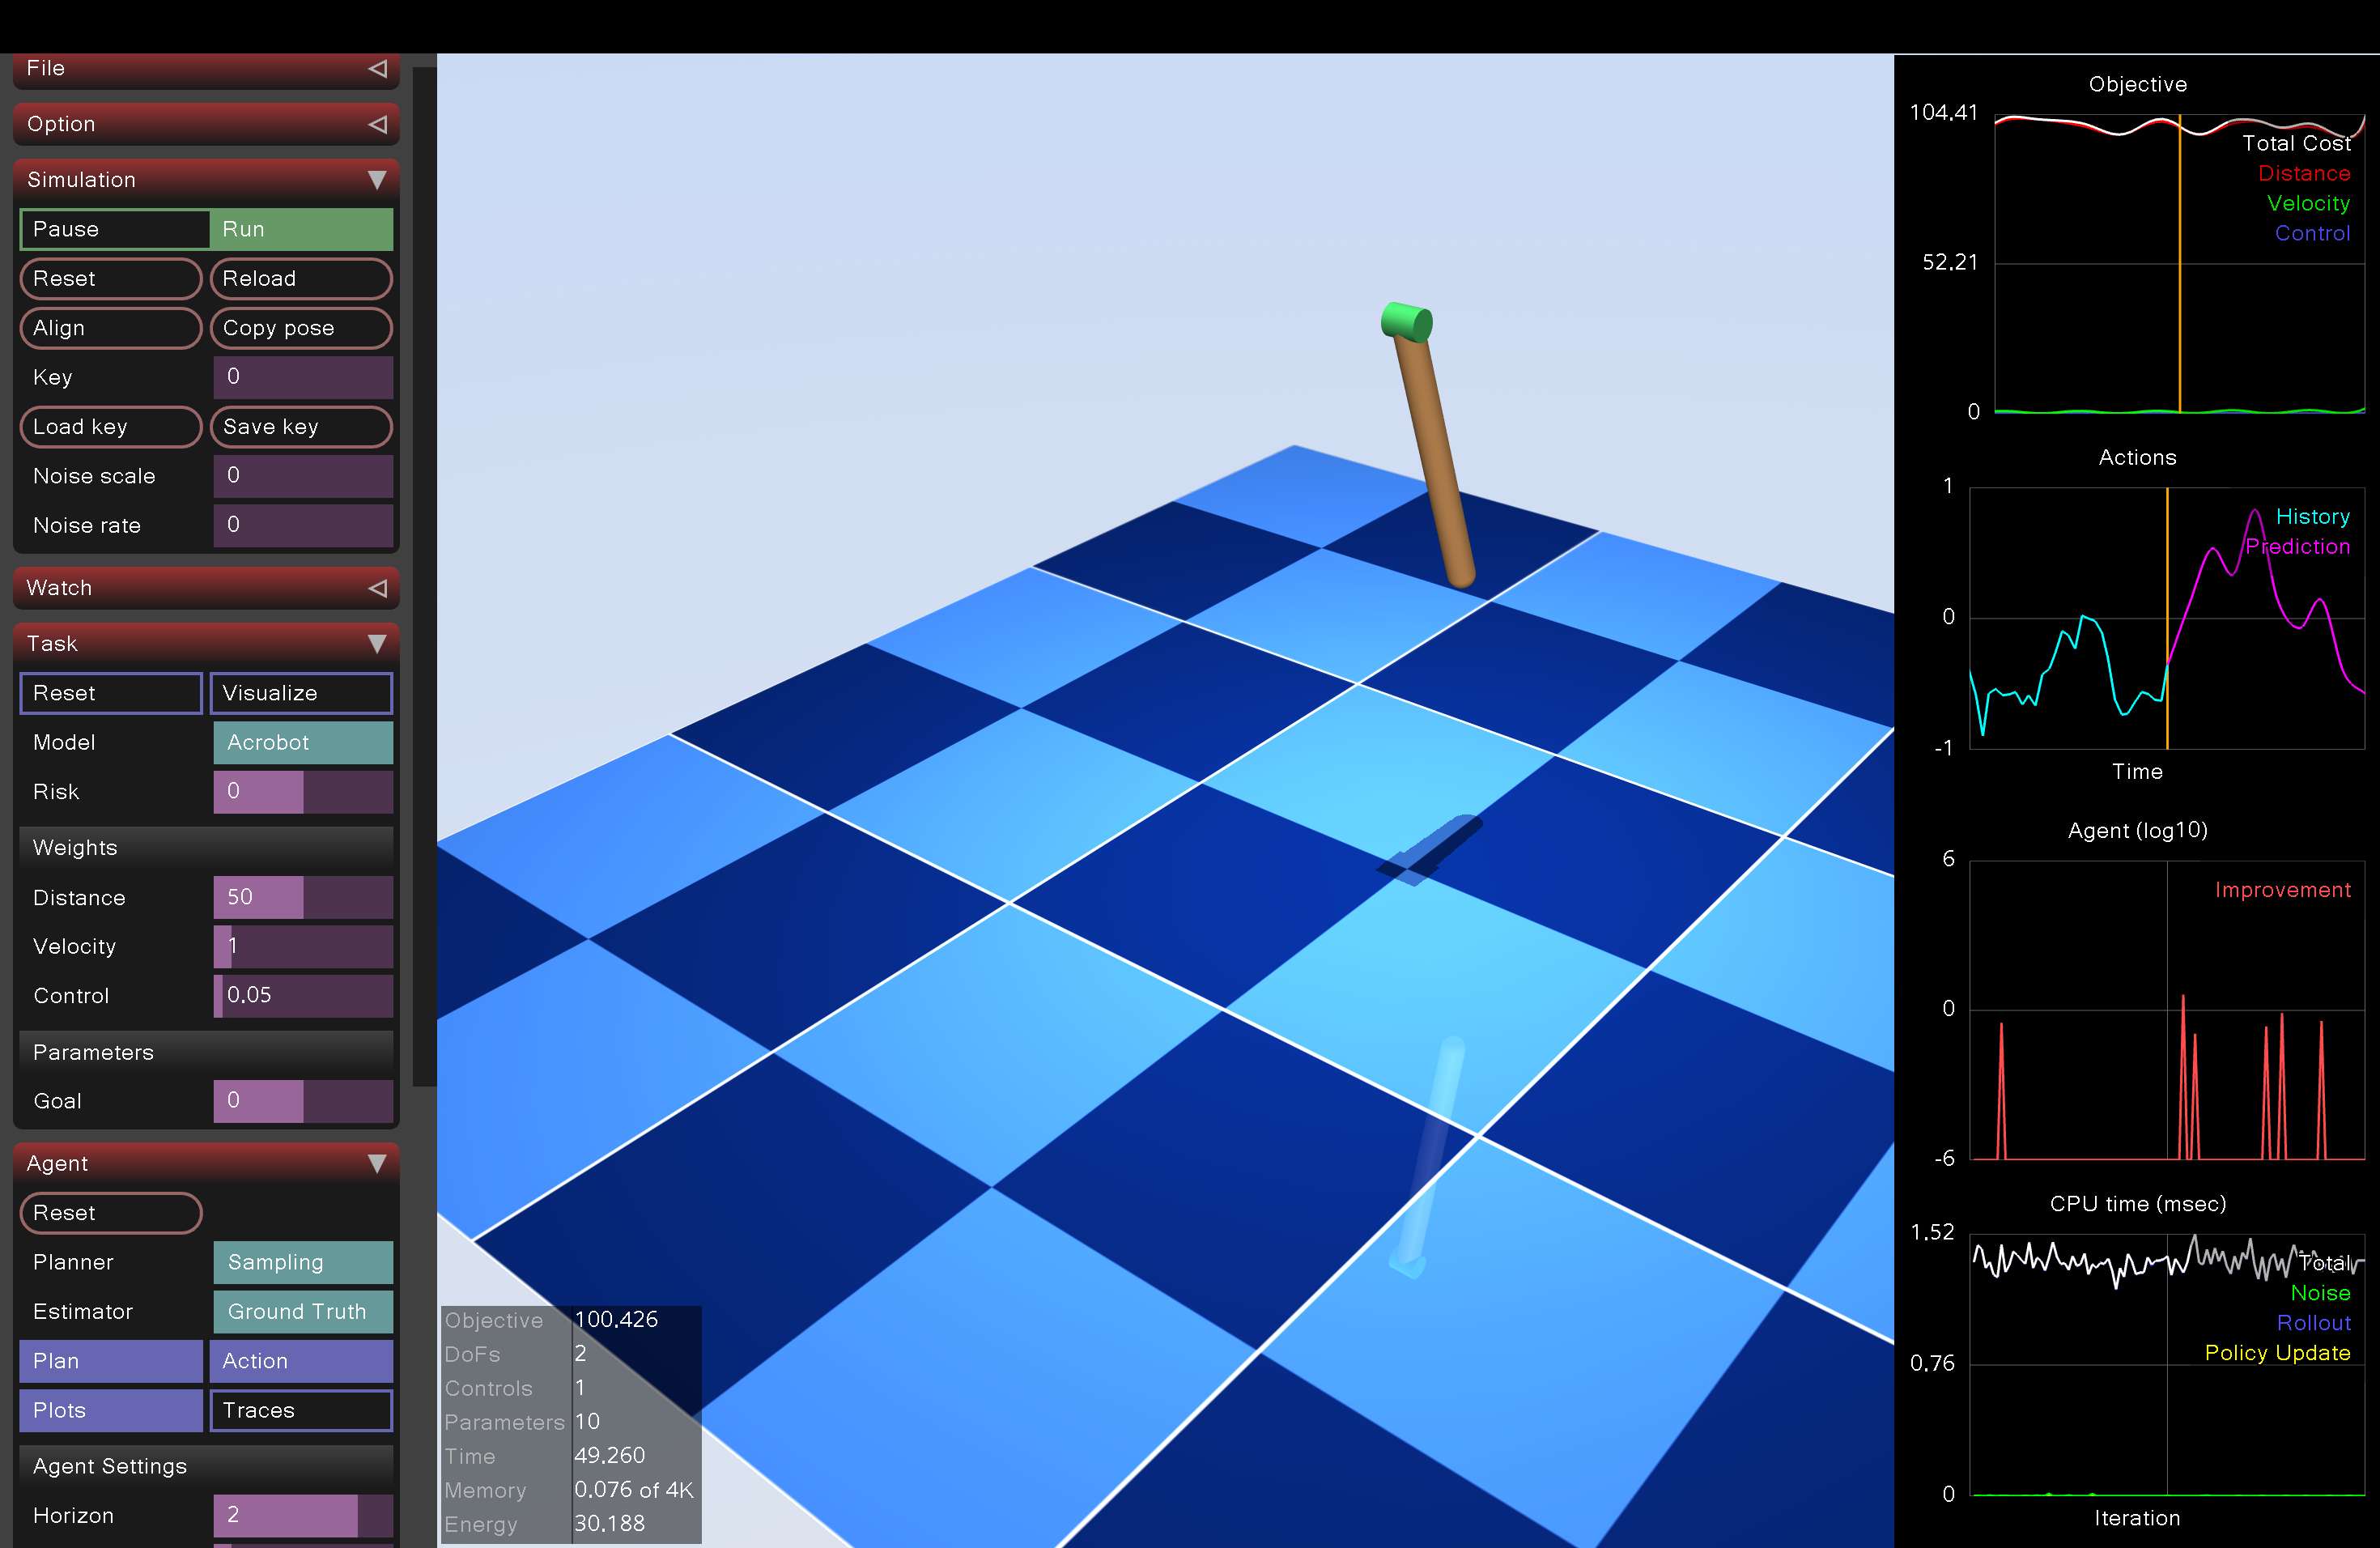
\includegraphics[width=0.46\textwidth]{p1/acrobot.png} \\
(a) Cartpole, Gradient planner & (b) Acrobot, Sampling planner \\[4pt]
\multicolumn{2}{c}{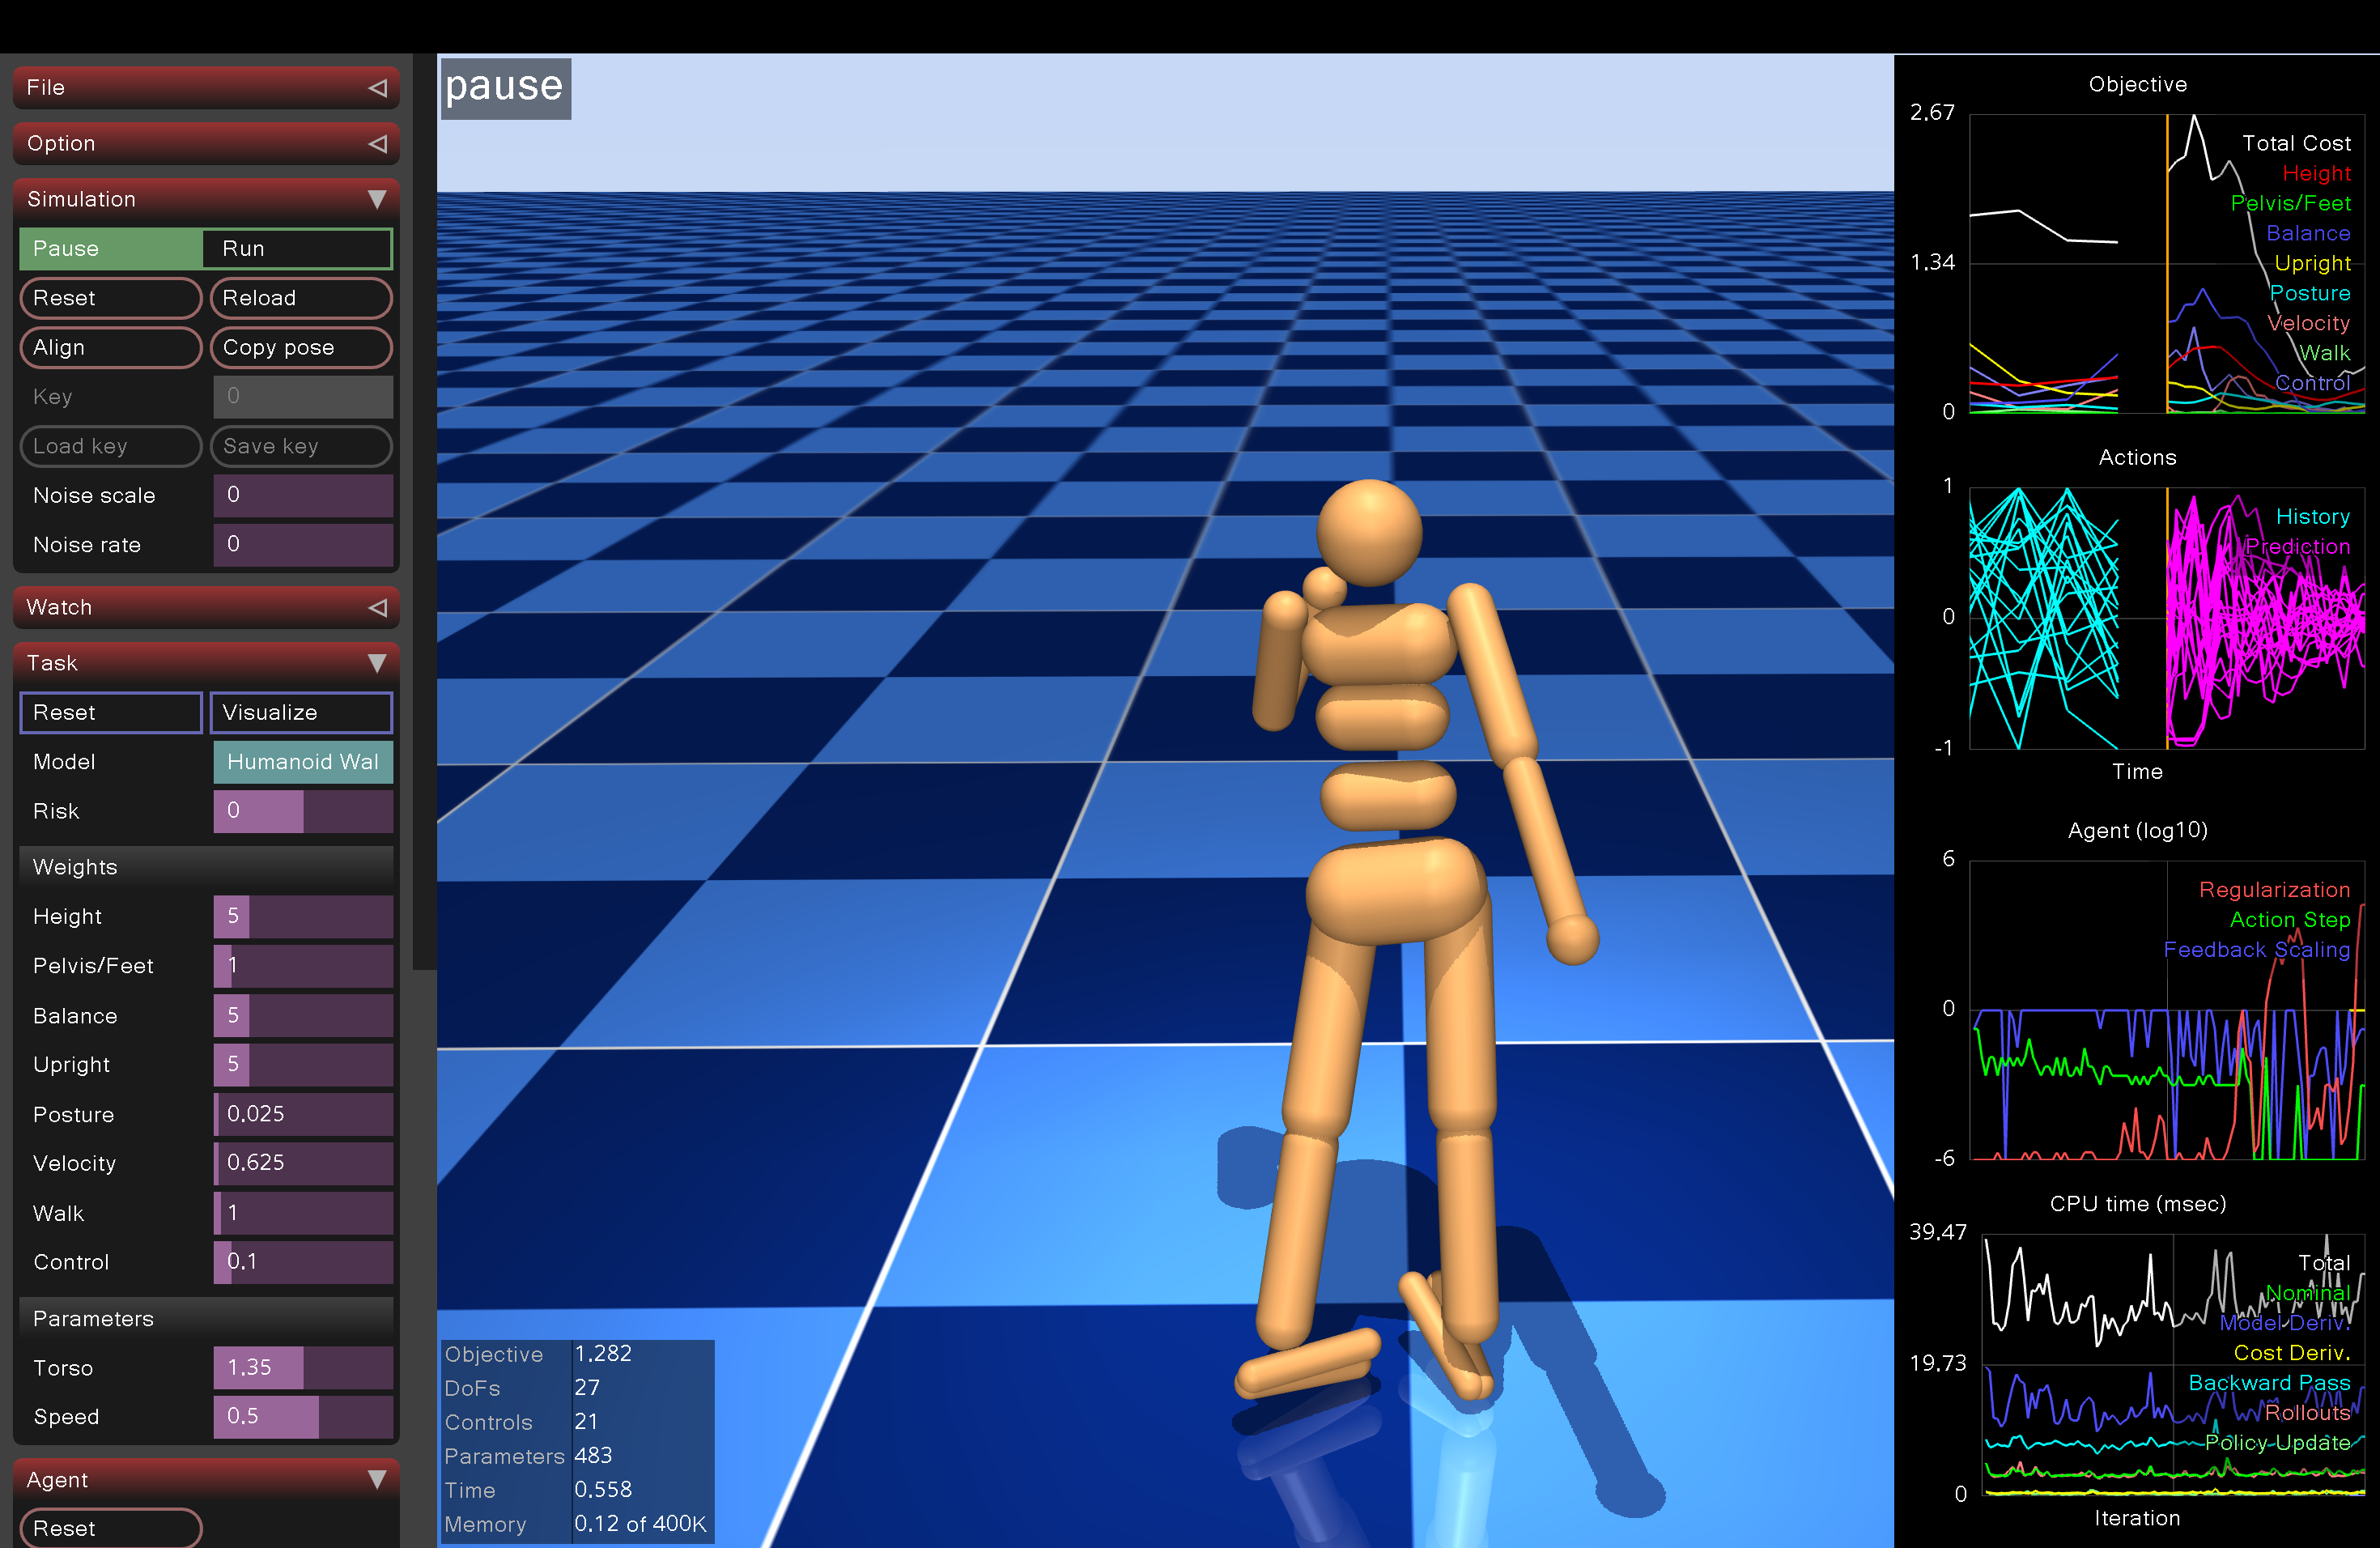
\includegraphics[width=0.6\textwidth]{p1/humanoid_walk.png}} \\
\multicolumn{2}{c}{(c) Walker (humanoid walk), Sampling planner} \\
\end{tabular}
\caption{MJPC controlling the three required systems. Right-side
panels show total cost (top), actions (middle) and planner internals
(bottom) over a sliding window.}
\label{fig:mjpc-3systems}
\end{figure}

\subsection*{(c) Humanoid Stand}
For the \texttt{humanoid\_stand} task we used the \emph{Sampling}
planner with $\texttt{Risk}=0$ and increased the relative weight on
the \texttt{Height} cost term (set to $100$) and the \texttt{Balance}
term so that the planner heavily prioritises keeping the centre of
mass at the target height before refining posture. We left
\texttt{Joint Vel.}\ and \texttt{Control} weights low to allow vigorous
corrective actions. Under these settings, the total cost drops to
$\approx 0.12$ and the humanoid maintains an upright stance for
the duration of the simulation; Fig.~\ref{fig:humanoid-stand} shows
the converged pose.

\begin{figure}[h]
\centering
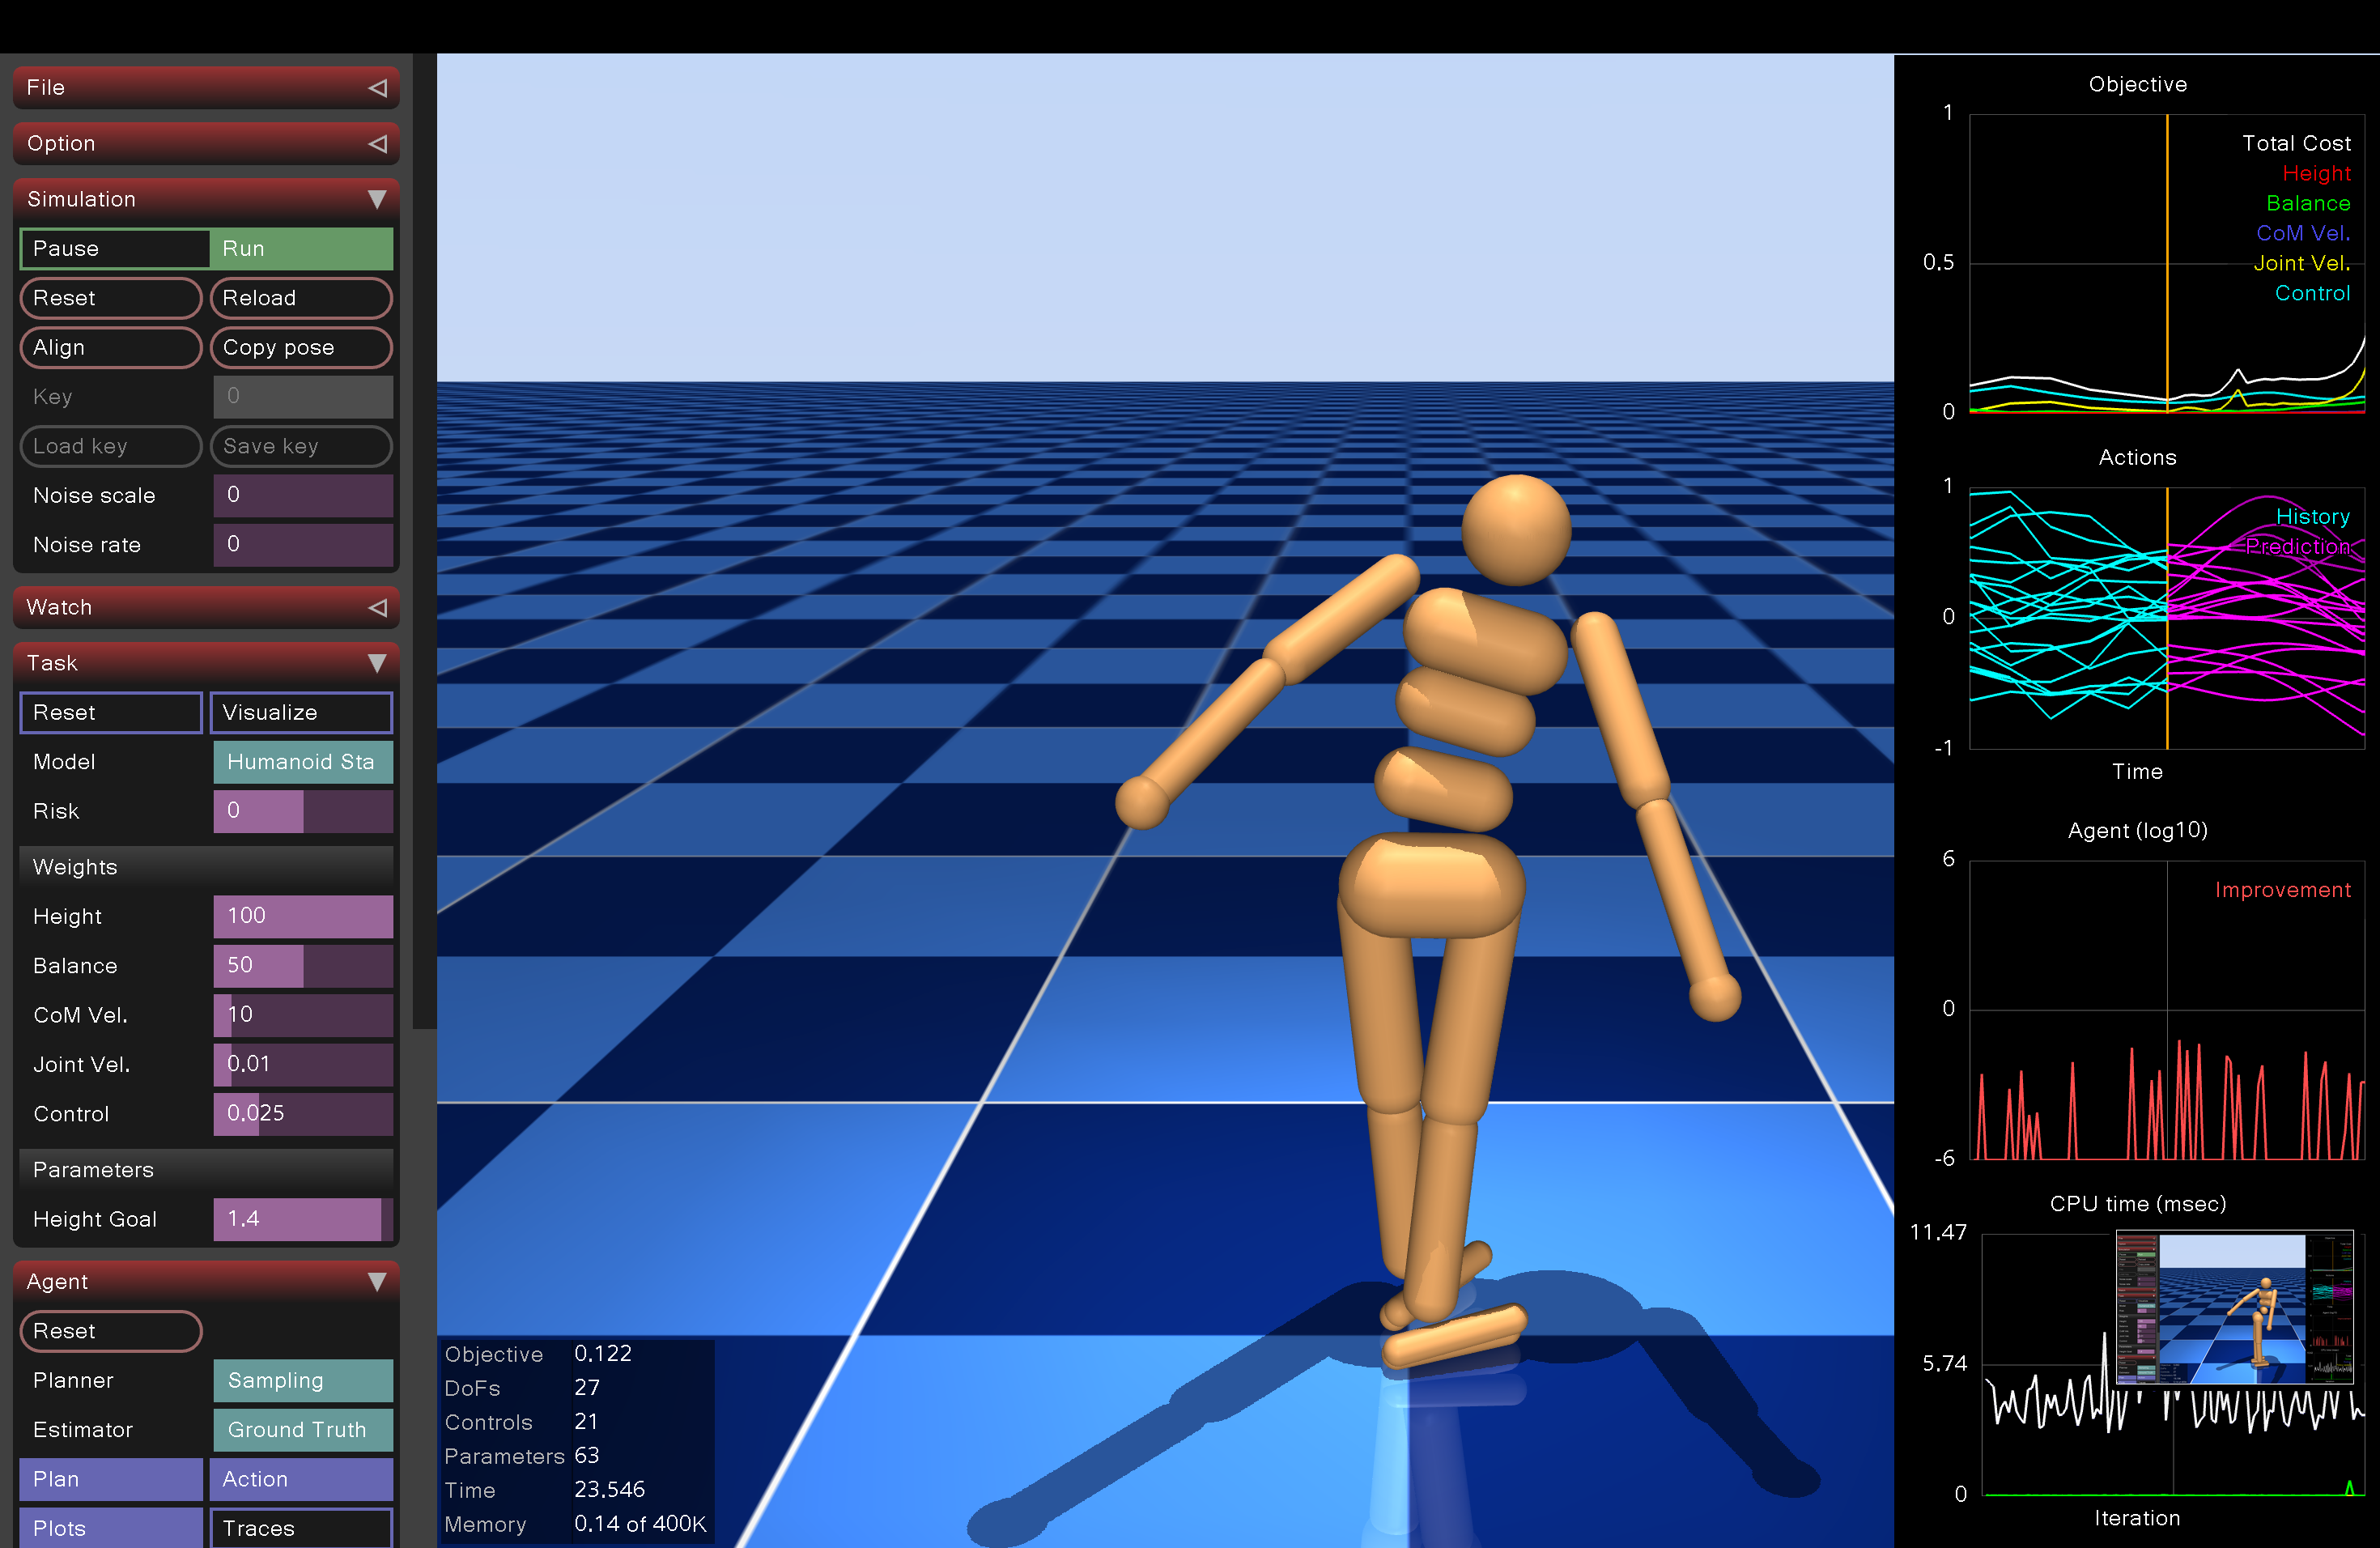
\includegraphics[width=0.7\textwidth]{p1/humanoid_stand.png}
\caption{Humanoid Stand task with tuned cost weights (\texttt{Height}=100,
emphasis on \texttt{Balance}). Total cost has settled near $0.12$,
indicating a stable upright equilibrium.}
\label{fig:humanoid-stand}
\end{figure}

\clearpage
%==============================================================================
\section{Problem 2 --- PPO for the DM Control Walker (75 pts)}

\subsection{Setup (a)}
We use the DeepMind Control Suite walker environment, \texttt{walker--walk}.
The state is a 24-D vector formed by concatenating:
\[
x = [\,\text{orientations}_{14}\,;\,\text{height}_{1}\,;\,\text{velocity}_{9}\,].
\]
The action is a 6-D vector of joint torques in $[-1, 1]$. The simulator
returns a per-step reward $r_t \in [0, 1]$ and a discount.

\paragraph{Stochastic controller.} We parameterise the policy as a
diagonal-Gaussian:
\[
u_\theta(u\mid x) = \mathcal{N}\bigl(\mu_\theta(x),\, \mathrm{diag}(e^{\log\sigma}\bigr)^2),
\]
where $\mu_\theta$ is a 2-layer ReLU MLP (hidden 256) and
$\log\sigma\in\mathbb R^6$ is a state-independent learnable parameter
initialised at $-0.5$ and clamped from below at $-1.0$ to keep the
policy stochastic. The actor input is the \emph{normalised} observation
(running mean/std). At rollout we sample $u\sim u_\theta(\cdot\mid x)$,
clip to $[-1, 1]$, and record the log-likelihood.

\subsection{PPO Implementation (b)}

\paragraph{Networks.} Two separate MLPs with orthogonal init (gain
$\sqrt 2$ on hidden layers, $0.01$ on the actor output, $1.0$ on the
critic output, biases zeroed):
\begin{itemize}[leftmargin=*,itemsep=0pt]
\item Actor:  $24 \to 256 \to 256 \to 6$ (ReLU); $\log\sigma$ is a
      free parameter shared across states.
\item Critic: $24 \to 256 \to 256 \to 1$ (ReLU).
\end{itemize}

\paragraph{Observation normalisation.} A running Welford estimator
maintains per-dimension mean/var of the raw 24-D observation. After
each rollout we (i) update the estimator with the new states and
(ii) symmetrise mean/var across the left/right mirror permutation
so that $\textsf{mirror}(\textsf{normalize}(x)) =
\textsf{normalize}(\textsf{mirror}(x))$.

\paragraph{Advantage (GAE-$\lambda$).} For each episode we compute
the truncated generalised advantage estimate
\[
\delta_t = r_t + \gamma V(x_{t+1}) - V(x_t),
\qquad
\hat A_t = \sum_{k\ge 0} (\gamma\lambda)^k \delta_{t+k},
\]
with $\gamma = 0.99$, $\lambda = 0.95$. For the last step of an episode
that ended on $r.\textsf{last}()$, $V(x_{T+1}) := 0$; otherwise we
bootstrap with $V(x_T)$. Targets for the critic are
$\hat G_t = \hat A_t + V(x_t)$. After concatenation across all episodes
in a batch the advantages are normalised (mean/std).

\paragraph{Loss.} The clipped surrogate plus auxiliary terms:
\[
L = \underbrace{-\mathbb E\!\left[\min\!\Bigl(\rho_t \hat A_t,\;
\mathrm{clip}(\rho_t,\,1-\varepsilon,\,1+\varepsilon)\,\hat A_t\Bigr)\right]}_{\text{PPO clip}}
\;-\; c_e \mathcal H[u_\theta]
\;+\; c_\pi^{\text{sym}} L^{\text{sym}}_\pi,
\]
\[
L_V = \tfrac12\,\mathbb E\!\left[\max\!\bigl((V_\theta - \hat G)^2,\,
(V_\theta^{\text{clip}} - \hat G)^2\bigr)\right]
\;+\; c_V^{\text{sym}} L^{\text{sym}}_V,
\quad
V_\theta^{\text{clip}} = V_\theta^{\text{old}} + \mathrm{clip}(V_\theta - V_\theta^{\text{old}},\,\pm\varepsilon_V).
\]
The mirror-symmetry regularisers exploit the bilateral symmetry of the
walker --- swapping the left and right limbs in the state should swap
the corresponding actions, and the value should be invariant:
\[
L^{\text{sym}}_\pi = \mathbb E\!\left[\bigl\|\mu(x) - \textsf{mirror}_a(\mu(\textsf{mirror}_x(x)))\bigr\|^2\right],
\quad
L^{\text{sym}}_V = \mathbb E\!\left[(V(x) - V(\textsf{mirror}_x(x)))^2\right].
\]
Implementation: \texttt{STATE\_PERM} and \texttt{ACTION\_PERM} encode
the L$\leftrightarrow$R swap of orientations, joint velocities, and
hip/knee/ankle actuators.

\paragraph{Training loop.} Each iteration:
(i) collect a batch of $\geq 8000$ environment steps across one or
more episodes; (ii) compute GAE; (iii) normalise advantages;
(iv) run \emph{10 epochs} of mini-batch SGD over the batch
(mini-batch $= 256$), with KL early-stop when
$\mathrm{KL}(\theta,\theta_\text{old}) > 1.5 \times$ target;
(v) clip gradients to global $\ell_2$-norm 0.5; (vi) anneal both
learning rates linearly from $3\times 10^{-4}$ down to $0$ over the
training budget. Best-by-batch-mean-return checkpoint is saved
continuously. Total budget: $3\times 10^{6}$ environment steps.

\paragraph{Hyperparameters.}
\begin{center}
\begin{tabular}{lll}
\toprule
$\gamma$, $\lambda$ & 0.99, 0.95 & discount, GAE \\
$\varepsilon$, $\varepsilon_V$ & 0.2, 0.2 & policy / value clip \\
LR (annealed) & $3\times 10^{-4} \to 0$ & Adam, $\epsilon=10^{-5}$ \\
target KL & 0.02 & inner-loop early-stop \\
batch / mini-batch & 8000 / 256 & per iteration \\
inner epochs & 10 & per iteration \\
hidden size & 256 & both nets, ReLU \\
$\log\sigma_0$ / clamp & $-0.5$ / $\geq -1.0$ & policy std \\
entropy coef $c_e$ & $5\times 10^{-3}$ & exploration bonus \\
sym coef $c_\pi^{\text{sym}}$, $c_V^{\text{sym}}$ & 0.5, 0.1 & mirror-symmetry \\
grad clip & 0.5 & global $\ell_2$-norm \\
total timesteps & $3\times 10^{6}$ & meets $\geq 10^6$ requirement \\
$T_{\max}$ & 1000 & dm\_control episode cap \\
\bottomrule
\end{tabular}
\end{center}

\paragraph{Differences from Spinning Up.}
\begin{itemize}[leftmargin=*,itemsep=0pt]
\item \textbf{Single-process rollouts.} Spinning Up uses MPI; we
      collect sequentially in one process.
\item \textbf{Mirror symmetry regulariser.} Specific to bipedal
      walkers: encoding L$\leftrightarrow$R symmetry as an auxiliary
      loss on both $\pi$ and $V$ dramatically accelerates learning a
      stable gait, since half the policy can be tied to the other half.
\item \textbf{Running observation normalisation} with symmetric mean/var.
\item \textbf{Value-function clipping}, \textbf{gradient clipping},
      and \textbf{LR annealing} for stability over multi-million step
      training.
\item \textbf{Entropy bonus} prevents the early collapse to deterministic
      policies that we observed without it.
\end{itemize}

\subsection{Results (b)}

Per-episode and 60-episode moving-average undiscounted episode return
are shown in Fig.~\ref{fig:returns}. With the design described above,
PPO improves smoothly from a first-100-episode mean of $53.6$ to a
final-100-episode mean of $\mathbf{926.9}$ (peak single-episode return
$980.8$ out of a theoretical max of $1000$). The trajectory has three
visible phases:
\begin{itemize}[leftmargin=*,itemsep=0pt]
\item \textbf{Standing-up} (0 -- 0.3M): the walker learns not to fall
      over immediately; mean return rises from $\sim50$ to $\sim250$.
\item \textbf{Gait emergence} (0.3M -- 1.5M): the symmetry regulariser
      ties left and right limb actions and a periodic walking gait
      emerges; mean return rises through $\sim500$ and the
      moving-average crosses $700$ around 1.8M.
\item \textbf{Refinement} (1.5M -- 3M): with the LR annealing schedule
      and the running observation normaliser stabilising the input
      distribution, the policy refines into a robust gait at
      $\bar G \approx 920\!-\!940$. Mean returns over the three windows
      $[0.2\text{M}, 0.5\text{M}]$, $[0.5\text{M}, 1.5\text{M}]$,
      $[1.5\text{M}, 3\text{M}]$ are $246.7,\ 532.7,\ 844.8$
      respectively.
\end{itemize}
Most full-length 1000-step episodes succeed; the per-episode trace
shows occasional sharp drops during the gait-emergence phase
corresponding to falls, but these become rare after 2M steps.

\begin{figure}[h]
\centering
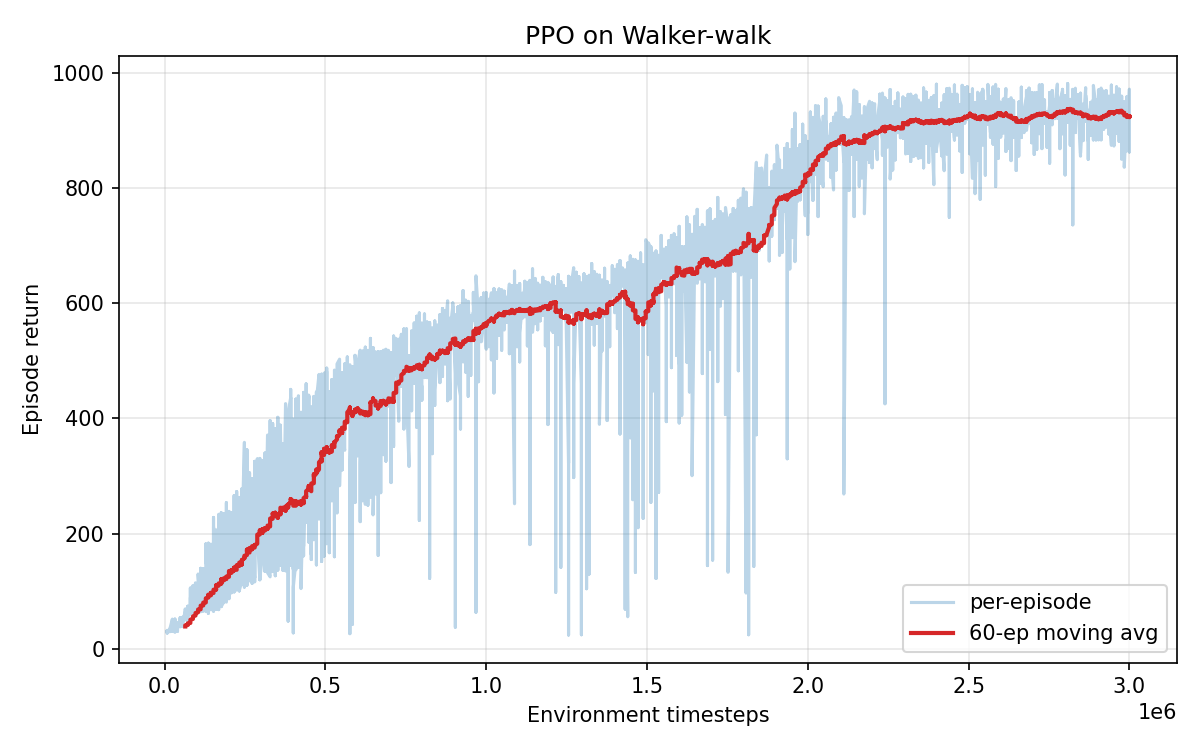
\includegraphics[width=0.78\textwidth]{p2/ppo_returns.png}
\caption{Mean undiscounted episode return per epoch versus environment
timesteps for PPO on \texttt{walker--walk}.}
\label{fig:returns}
\end{figure}

\paragraph{Walker rollout frames.} The trained best-checkpoint policy
(\texttt{actor.pt}) was rolled out in the DM Control walker environment
using deterministic mean actions (with observation normalisation
applied), and frames were rendered offscreen via
\texttt{physics.render}. The 800-step evaluation episode return was
$\mathbf{775.2}$, consistent with the training-time moving average
($\sim 925$) given that this single roll-out uses a deterministic
policy and a fresh seed.

\begin{figure}[h]
\centering
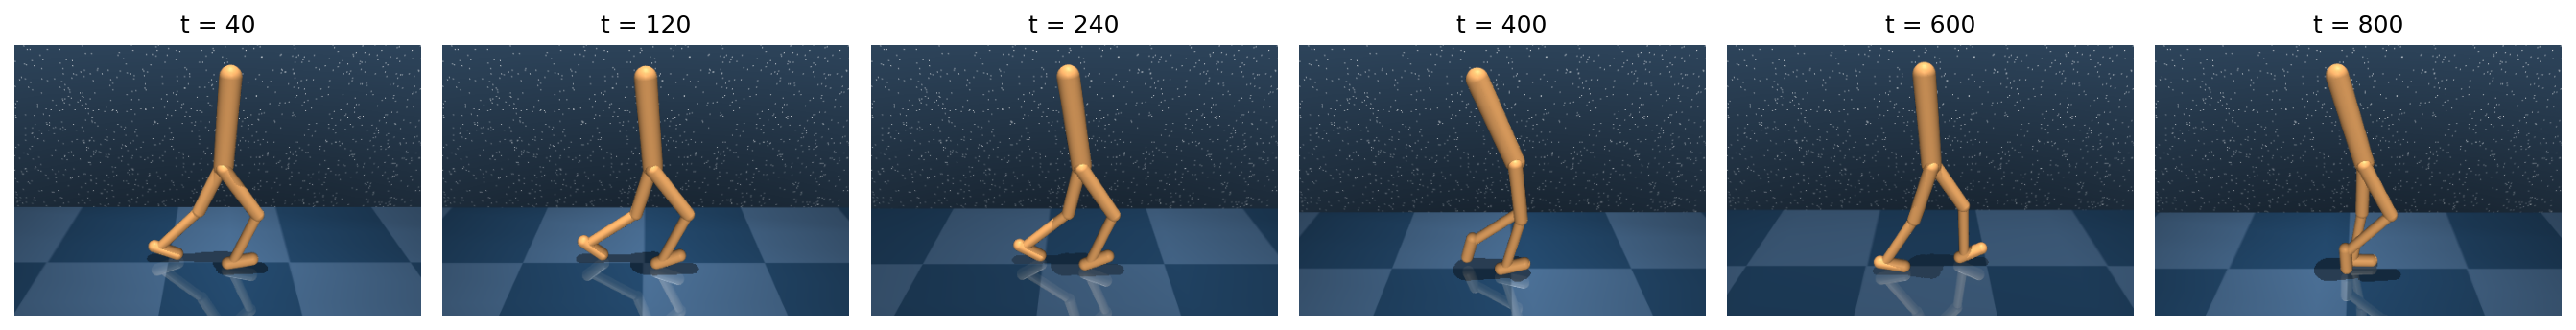
\includegraphics[width=\textwidth]{p2/walker_strip.png}
\caption{Trained walker rolled out for 800 simulator steps with the
deterministic mean policy. Frames captured at
$t = 40, 120, 240, 400, 600, 800$ (offscreen render). The torso stays
upright and the legs alternate, exhibiting a stable bipedal walking
gait.}
\label{fig:walker_strip}
\end{figure}

\subsection{Discussion}

\paragraph{Why GAE-$\lambda$.} A first iteration of this implementation
used Spinning Up's "single-sample Monte Carlo return-to-go" shortcut as
a proxy for $Q$. With this estimator the $\hat A$ signal was noisy enough
that $\bar G$ plateaued around $\approx 100$ (out of a possible $1000$)
and the resulting walker could not stand without policy noise. Switching
to truncated GAE-$\lambda$ ($\lambda = 0.95$) trades a small bias for a
large variance reduction and was the single most important change to
unlock learning beyond a few hundred return.

\paragraph{Mirror-symmetry regulariser.} The dm\_control planar walker
is bilaterally symmetric: swapping the left and right hip/knee/ankle
state coordinates and the corresponding actions leaves the dynamics
and reward unchanged. We expose this prior to PPO as a soft auxiliary
loss on both the policy mean and the value function (coefficients $0.5$
and $0.1$ respectively). In practice this halves the effective sample
complexity and yields a noticeably smoother gait.

\paragraph{Observation normalisation.} A whitened state input keeps the
network input distribution roughly stationary across training despite
the running mean/var changing as the policy explores new regions.
Whitening is symmetrised (mean/var averaged with their L$\leftrightarrow$R
mirrored counterparts) so the symmetry regulariser is consistent with the
normaliser.

\paragraph{Value clipping + grad clipping + LR annealing.} These three
keep the optimisation stable across multi-million-step training. Without
value clipping, the critic would occasionally swing by a large amount
between mini-batches and corrupt the next iteration's GAE signal.

\clearpage
\appendix

\section{Source code: \texttt{18330723\_hw4\_p2.py}}
\label{app:main}
The main PPO trainer. Contains the actor / critic networks, observation
normaliser, GAE roll-out, mirror-symmetry helpers, and the training and
evaluation entry points.
\lstinputlisting[style=appendixsrc]{p2/18330723_hw4_p2.py}

\clearpage
\section{Source code: \texttt{render\_frames.py}}
\label{app:render}
Offscreen roll-out and PNG strip generator used to produce
Fig.~\ref{fig:walker_strip} (no GUI required).
\lstinputlisting[style=appendixsrc]{p2/render_frames.py}

\clearpage
\section{Source code: \texttt{view.py}}
\label{app:view}
Thin launcher that loads the trained checkpoint and the observation
normaliser, then opens the dm\_control \texttt{viewer} for interactive
inspection.
\lstinputlisting[style=appendixsrc]{p2/view.py}

\end{document}
